\section{MIP}\label{sec:mip}

\subsection{Tri-linear Interpolation}\label{sec:tri_linear}
- added function getTriVoxel

\begin{figure}[h!]
    \centering
    \captionsetup{justification=centering,margin=0.5cm}
    \begin{subfigure}[t]{0.48\textwidth}
        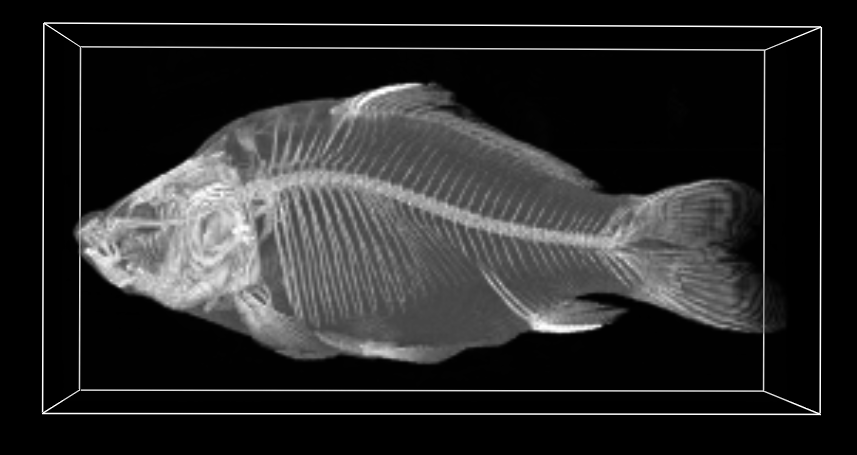
\includegraphics[width=\textwidth]{img/fish_NN.png}
        \caption{ }
    \end{subfigure}
    \begin{subfigure}[t]{0.48\textwidth}
        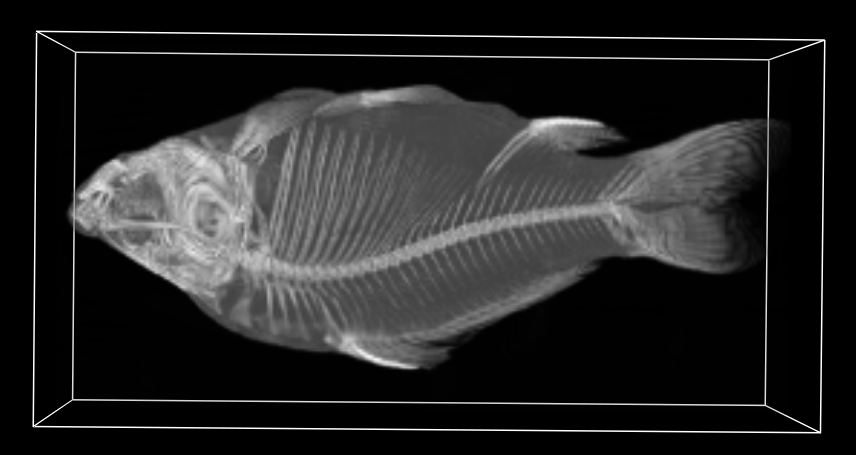
\includegraphics[width=\textwidth]{img/fish_TriLin.png}
        \caption{ }
    \end{subfigure}
    \caption{difference between NN interpolation and Tri-Linear interpolation}
    \label{fig:trilinear}
\end{figure}

\subsection{Performance Enhancing}\label{sec:perf_enh}

- took location calculation for i and j out of the for-loop
- let loop break when a value of 255 is already found (can't get any higher) (does not work for composite!?)
- todo: stop the walk along a ray when it comes out of the bounding box. 